\section{Segmentation of Myotubes with \texttt{MyoSAM}}\label{secsam}

Myotube and cell nuclei microscopy images significantly differ from natural images. While cell nuclei images tend to be more homogeneous in size and shape of the nuclei, presenting recurring problems, myotube images exhibit far greater diversity. Our exploratory data analysis aimed to understand the characteristics of myotube images, both quantitatively and qualitatively.

\paragraph{Qualitative Analysis}
\begin{figure}
	\centering
	\includegraphics[width=\textwidth]{"images/myotube_image_set.png"}
	\caption[Sample myotube images]{Sample of myotube images of varying sizes.}
	\label{figsamplemyotubes}
\end{figure}
\ \\
In the myotube image set eventually used for training, it is clear that the images vary widely in size, brightness, and color schemes. They are primarily monochromatic, with their color depending on the biomarker used and the type of microscope employed for capturing the images (cf. Fig.~\ref{figsamplemyotubes}). Additionally, the myotubes themselves display considerable variation in size, shape, and density. This variety underscores the diverse data distribution present within myotube images as a whole.

\paragraph{Quantitative Analysis}
\ \\
Upon evaluating the images selected for training, we found that myotube images are predominantly dark. The evaluated images had average red, green, and blue values of 2.56, 9.8, and 2.9, respectively, with a high degree of variance. Further analysis into the HSL (Hue, Saturation, Lightness) space of these images confirmed their darkness, primarily attributed to the large areas of dark background present. Fig.~\ref{figrgb}, Fig.~\ref{fighsl} and the table below summarize the activations for red, green, blue, and lightness across several images.

\begin{tabular}{|p{2cm}|p{2cm}|p{2cm}|p{2cm}|p{2cm}|p{2cm}|}
	\hline
	& Minimum Activation & Minimum non-zero  activation & Maximum activation & Mean of mean activations & Mean of activation standard deviations \\
	\hline
	Red & 0 & 1.89 & 6.90 & 2.56 & 3.88 \\
	\hline
	Green & 0 & 1.89 & 28.34 & 9.79 & 8.13 \\
	\hline
	Blue & 0 & 2.84 & 17.48 & 2.90 & 2.36 \\
	\hline
	Lightness & 0.64 & NA & 14.23 & 5.37 & 4.75 \\
	\hline
\end{tabular}

\begin{figure}
	\centering
	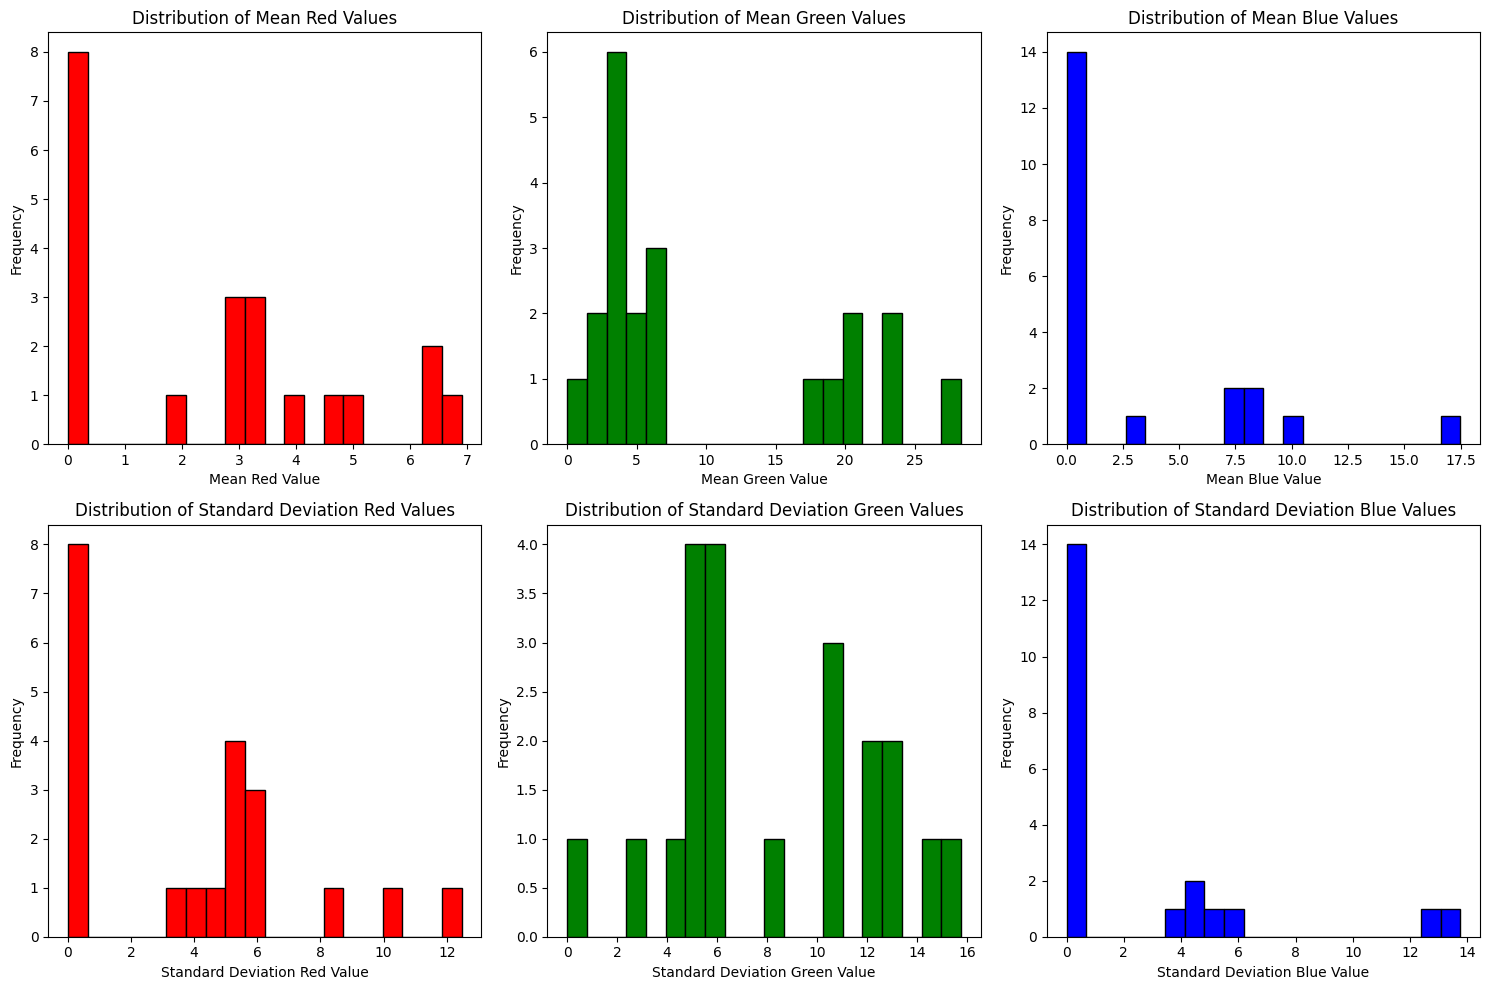
\includegraphics[width=\textwidth]{"images/pixel_distribution_plots_rgb.png"}
	\caption[Myotube RGB activation distribution]{Activation of RGB channels in the myotube training dataset.}
	\label{figrgb}
\end{figure}
\begin{figure}
	\centering
	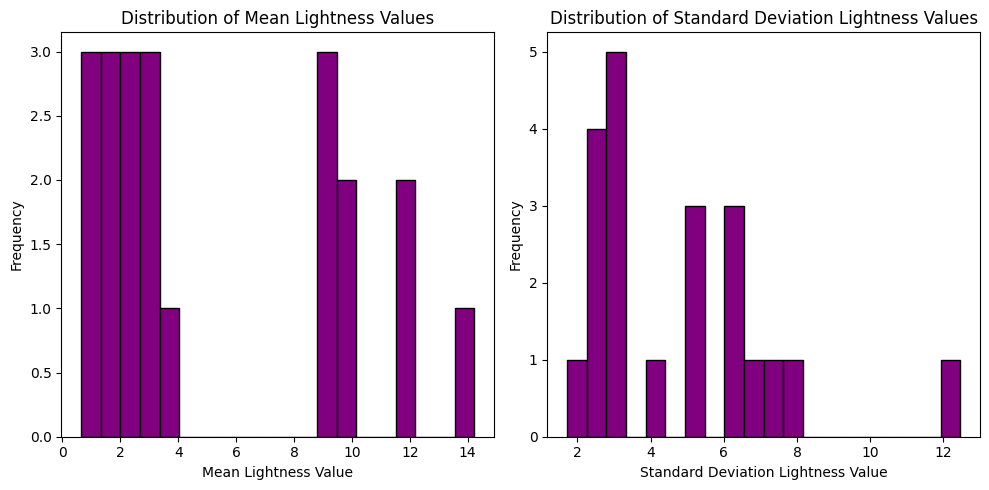
\includegraphics[width=\textwidth]{"images/pixel_distribution_plots_hsl.png"}
	\caption[Myotube lightness activation distribution]{Activation of lightness channel from HSL space in the myotube training dataset.}
	\label{fighsl}
\end{figure}
\ \\
This analysis highlights the necessity of treating myotube images differently from natural images. For instance, typical normalization techniques based on pixel activation means derived from natural images are not directly applicable to myotube images due to their unique characteristics.

Alas, typical myotubes cannot be represented as star-convex polygons since oftentimes they have slight constrictions (cf. Fig.~\ref{figtubeblast}) or even bifurcations.

Recently, the Segment Anything Model (SAM) \cite{kirillov2023segment} developed by Meta AI has demonstrated great promise in the field of natural image segmentation. Trained on the largest segmentation dataset to date, encompassing over 11 million diverse images and 1 billion corresponding masks, this model benefits from both the scale and quality of the dataset. With its powerful transformer-based architecture, \texttt{SAM} has gained a comprehensive understanding of objects, enabling it to achieve exceptional zero-shot performances, sometimes even surpassing fully supervised models.
Despite the significant progress made within the zero-shot framework, challenges arise when applying \texttt{SAM} to more specialised domains such as medical and satellite imaging. Due to the underrepresentation of images from these domains in the training data, the model is not as precise as desired. For instance, as illustrated in Fig.~\ref{figzeroshot}, \texttt{SAM} struggles with identifying overlapping myotubes. Moreover, in scenarios where segmentation of only specific critical areas is required, using \texttt{SAM} can be overwhelming as it attempts to “segment anything” it detects, including background, small artifacts, small nuclei cells within myotubes, and edges of the image. To address these challenges and enable a fully automatic instance segmentation process, fine-tuning the model was necessary, leading to a model we dubbed Myovision Segment Anything Model (\texttt{MyoSAM}).

\begin{figure}
	\centering
	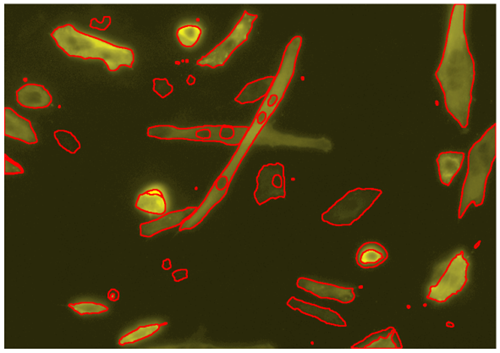
\includegraphics[width=\textwidth]{"images/sam_zeroshot.png"}
	\caption[\texttt{SAM} zeroshot]{Out-of-box application of the pretrained version of \texttt{SAM} to one patch of a myotube image.}
	\label{figzeroshot}
\end{figure}
\subsection{\texttt{SAM} Background}\label{SAMbg}
The strong generalization capability of the \texttt{SAM} was achieved through careful design of its task objective, model architecture, and dataset used in training. The goal of the Meta AI research team was to develop a model capable of generalizing across various downstream computer vision tasks and data distributions, including instance segmentation, edge detection, and object suggestions, among others.

Meta AI's reserchers drew inspiration from how humans would perform the aforementioned tasks. Drawing parallels to the human ability to adapt to various tasks through acquired expertise within a specific domain, one would typically present a person with an image alongside some form of guidance on what is expected. This guidance could be a direct indication of the object to segment, such as pointing to it, creating boundaries around it with a box or a mask, or providing instructions in text form, especially when face-to-face communication isn't an option.

Initially, the human would discern and isolate the object, subsequently carrying out the tasks as directed. These guiding signals are termed “prompts“, a concept adapted from the field of Natural Language Processing (NLP). The Meta AI Research Team has termed this versatile task \textit{promptable segmentation task}. It involves providing an image and a prompt to produce a segmentation mask for the specified object, which then can be utilised for a variety of downstream tasks. However, there is an added layer of complexity: the model should be capable of formulating multiple segmentation masks from a single prompt. This is because prompts may be vague and potentially applicable to multiple objects within an image. For instance, a prompt might relate to a person, a bag, or even a zipper on the bag. Despite the ambiguity, the model is expected to generate at least one meaningful mask corresponding to one of the objects the prompt refers to.
Such a promptable segmentation task inevitably imposes specific constraints on the possible model architectures. The model must be capable of processing an image as input while simultaneously encoding various forms of prompts. It must then combine these two streams of information to accurately predict the segmentation mask. Additionally, the integration of image and prompt inputs must be designed efficiently in a fashion so as to allow real-time interactive segmentation. 
Meta AI devised a distinctly clear model architecture that satisfies all the outlined constraints effectively. The model consists of image encoder, prompt encoder, and a lightweight mask decoder. A high-level overview of \texttt{SAM} can be gained through Fig.~\ref{figsamoverview}.

The broad idea behind the model is simple: there needs to be a way to independently embed both prompt and image in order to jointly predict masks. The model therefore mainly consists of image encoder, prompt encoder, and a decoder network.
\begin{figure}
	\centering
	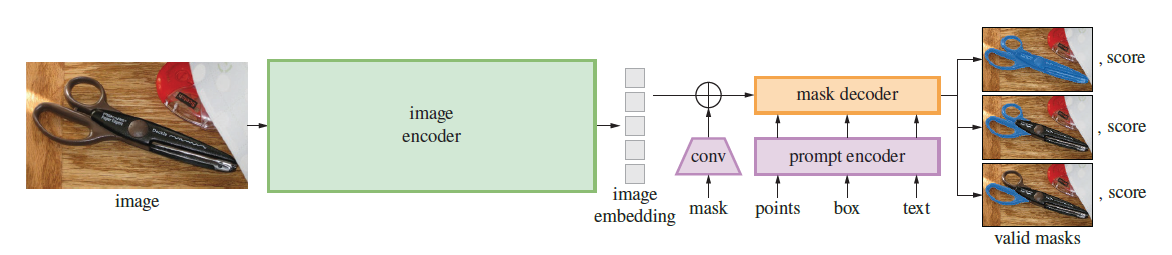
\includegraphics[width=\textwidth]{"images/sam_overview.png"}
	\caption[\texttt{SAM} Overview]{High-level overview of the two encoder networks interact to predict segmentation masks. Source: \cite{kirillov2023segment}.}
	\label{figsamoverview}
\end{figure}
A modified vision transformer \cite{dosovitskiy2020image} (ViT) is used as the image encoder. When applying ViTs the input image is divided into fixed-size patches. Each patch is embedded and treated as a token analogous to words in text tying in with the similarities to NLP. One dimensional positional encodings are added in order to retain spatial information. The image embeddings, along with positional encodings, are fed into a transformer encoder \cite{vaswani2017attention} consisting of attention blocks and feedforward neural networks, enabling the model to capture global dependencies between patches. Following the transformer encoder, the output is pooled to generate a fixed-size representation of the entire image, which is subsequently processed by fully connected layers for the final task. This approach offers benefits such as global context understanding, scalability to larger image sizes, and fewer inductive biases compared to traditional convolutional neural networks. Images are rescaled and padded to have a resoultuion of 1024x1024. The resulting image embedding output of the original vision transformer is of size 1280 x 64 x 64 and convolved twice to get to a size 256 x 64 x 64. 

While the image encoder is allowed to be computationally expensive since it only needs to be applied one time per image, both prompt encoder and mask decoder should be lightweight and fast to guarantee the ability to set many prompts and decode multiple masks at once. \texttt{SAM} allows for two types of prompts: sparse (text, boxes, points) and dense (masks) ones. As only point prompts were used in this work, only those will be discussed in the following and will simply be referred to as prompts. In order to encode the prompts, two pieces of information are required: foreground/background knowledge and positional knowledge. The positional encoding is either summed with an embedding for the foreground or one for background to form a 256 dimensional vectorial embedding.

Both types of embedding are then included into the decoder network. The decoder is depicted in Fig.~\ref{figdecoder} and its primary part consists of four steps. These four steps are performed twice to update both image and prompt embeddings. In addition to the prompt embeddings, an output token is introduced and their combinatation is then referred to as tokens. This is the only stage where there is any sort of information exchange between prompt and image. In the first step, self-attention is applied on the tokens. Afterwards the tokens are used as queries to compute the cross-attention to the image embeddings\footnote{Note that image embeddings go hand in hand with their positional embedings, too.}. As a third step, a multi-layer-perceptron (MLP) updates the tokens. Eventually, the complement of the second step is performed: the cross attention from image to tokens. The learned image embeddings, which are now aware of the prompt information, are upsampled through transposed convolutions and, at the same time, are attended to once more by the tokens. A 3-layer MLP is used to transform these tokens to a dimension so as to match the upscaled image embeddings. A pointwise product between this MLP's output and the upscaled image embeddings results in the prediction of the mask. The aforementioned output token is used within a second head to predict values for the intersection over union (IoU) to the ground truth. In order to remove ambiguity due to a given prompt, several (three by default) masks are predicted and ranked by their IoU scores. During training only masks with the highest IoU are used for the calculation of the loss.\footnote{As we only predict one mask per prompt, sorting by IoU was of little importance in this work.} 

It remains to discuss the training loop. Interactive segmentation is simulated during training by uniformly sampling a foreground point from the ground truth mask $G = (g_{i})$ and selecting subsequent points from the error region (both false positive and false negative) between the previous (binary) mask prediction $M$ and the ground truth, with each new point classified as foreground or background based on what type of error region $E$ it was sampled from. A mask prediction is provided from the previous iteration as an additional prompt, using unthresholded mask logits $P = (p_{i})$ to maximize information transfer. When multiple masks are returned, the one with the highest predicted IoU is used for the next iteration. After eight iteratively sampled points diminished returns are observed. Two additional iterations are included without new external information to allow the model to refine its predictions. One such iteration is performed at the very end and one is introduced after one randomly chosen iteration. The corresponding pseudocode can be found in App.~\ref{pcsam}. This results in a total of 11 iterations, balancing the use of external guidance with the model's own learning. This lightweight mask decoder allows for a relatively large number of iterations with minimal computational overhead compared to previous methods. The loss that is used is made up of three components: dice loss, focal loss \cite{liu2009otsu}, and IoU loss. The latter is just the penalization of the IoU prediction and is nothing but the mean squared error. The dice loss penalizes predictions by the percentage of misclassified pixels. The focal loss is a modification of the cross entropy loss with a modulation factor $\gamma$ to scale down the loss assigned to well-classified examples. All in all, the loss takes the form
\begin{equation}\label{samloss}
	L_{\text{train}} = L_{\text{dice}} + 20L_{\text{focal}}+ L_{\text{IoU}} = \left(1 - \dfrac{2|M \cap G|}{|M| + |G|}\right) - 20\sum_{i}(1-p^t_i)^{\gamma}\log p^t_i + \|\text{IoU}_{\text{pred}} - \text{IoU}_{\text{gt}}\|_{L^2}^{2},
\end{equation}
where $|\cdot|$ denotes the number of pixels of an area and the logits are defined as
\begin{equation*}
	p_i^\text{t}=\begin{cases}p&\text{if}\quad g_i=1\\1-p&\text{if}\quad g_{i}=0\end{cases},
\end{equation*}
and the summation runs over all pixels. $\gamma = 2$ was used during training.

\begin{figure}
	\centering
	\begin{subfigure}{0.45\textwidth}
		\centering
		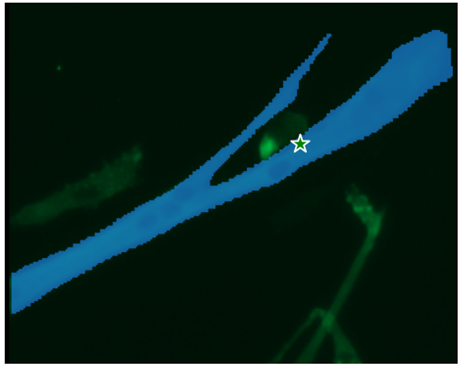
\includegraphics[width=\linewidth]{images/training1}
		\caption{First sampled foreground point from the ground truth mask}
		\label{figtrain1}
	\end{subfigure}
	\hfill
	\begin{subfigure}{0.45\textwidth}
		\centering
		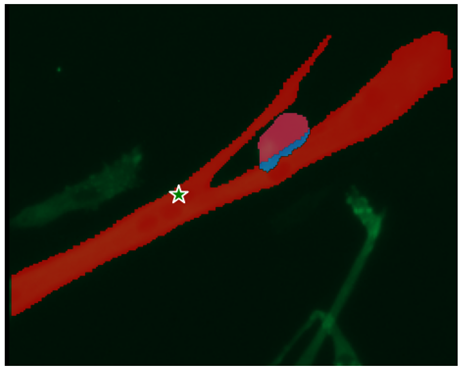
\includegraphics[width=\linewidth]{images/training2}
		\caption{Error region after the first prediction including new sampled (here: foreground) point}
		\label{figtrain2}
	\end{subfigure}
	
	\medskip
	
	\begin{subfigure}{0.45\textwidth}
		\centering
		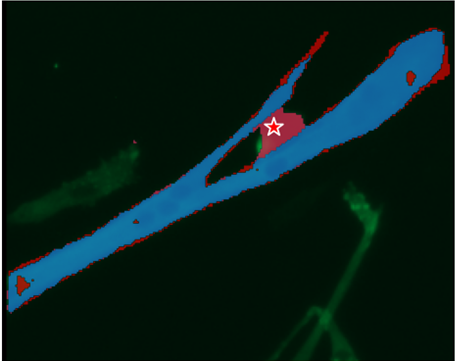
\includegraphics[width=\linewidth]{images/training3}
		\caption{New error region with another new (here: background) point prompt}
		\label{figtrain3}
	\end{subfigure}
	\hfill
	\begin{subfigure}{0.45\textwidth}
		\centering
		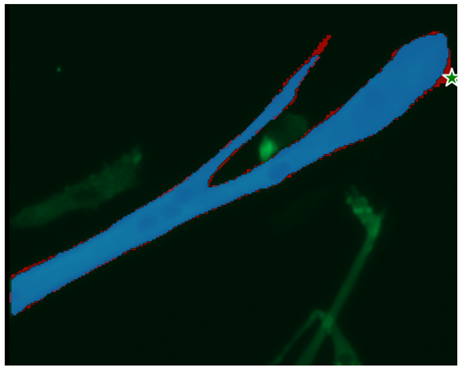
\includegraphics[width=\linewidth]{images/training4}
		\caption{Iteration beyond which resampling displays deminishing return}
		\label{figtrain4}
	\end{subfigure}
	\caption[\texttt{SAM} trainings loop]{Exemplifying the main idea behind the \texttt{SAM} training loop}
	\label{figtrain}
\end{figure}

\begin{figure}
	\centering
	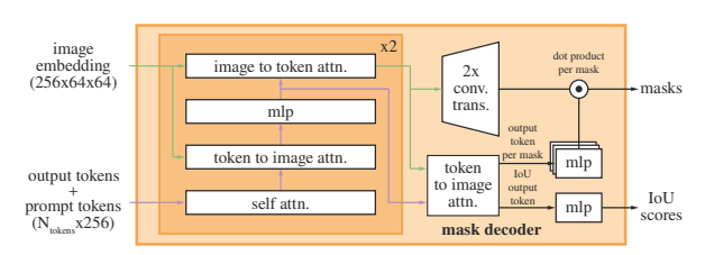
\includegraphics[width=\textwidth]{"images/maskdecoder.png"}
	\caption[\texttt{SAM} mask decoder]{Four attention steps in the mask decoder. Source: \cite{kirillov2023segment}.}
	\label{figdecoder}
\end{figure}

In order to provide a fully automated instance segmentation method without setting several prompts manually, the \texttt{SAM}AutomaticMaskGenerator class was created by Meta AI and introduced in the original publication \cite{kirillov2023segment}. This allows an instance of the class to automatically set the number of points per side, the number of crops performed before setting these points, NMS thresholds, and many other scores in order to get many masks at once.